\documentclass{beamer}

\usepackage[utf8]{inputenc}
\usepackage[danish]{babel}
\usepackage{tikz}
\usepackage{mathtools}
\usepackage{multirow}
\usepackage{anyfontsize}
\definecolor{Plum}{rgb}{0.56, 0.27, 0.52}
\usetikzlibrary{arrows}
\usetikzlibrary{calc}
\usetikzlibrary{decorations.markings}
\graphicspath{{../imgs/}}

\usetheme{Ilmenau}
\usecolortheme{beaver}
\uselanguage{Danish}
\languagepath{Danish}

\setbeamerfont{itemize/enumerate subbody}{size=\scriptsize}

\newcommand{\unit}[1]{\ensuremath{\:\text{#1}}}
\newcommand{\pro}{\ensuremath{\unit{\%{}}}}
\graphicspath{{../imgs/}}

\expandafter\def\expandafter\insertshorttitle\expandafter{%
  \insertshorttitle\hfill%
  \insertframenumber\,/\,\inserttotalframenumber}

\setbeamertemplate{itemize item}[square]
\setbeamertemplate{itemize subitem}[circle]
\setbeamertemplate{enumerate item}[square]

\title{DaLUKE}
\subtitle{
    Den danske sprogmodel med vidensmodellering
}
\author[Søren Holm, Asger Schultz]{Søren Winkel Holm og Asger Laurits Schultz}
\institute[DTU]{Danmarks Tekniske Universitet}
\date{7. juli 2021}

\begin{document}

\begin{frame}
    \titlepage
\end{frame}

%Kom hurtigt til resultater
%Relativt få slides
%Vis arbejde
%Understøt med figurer
%Evt demonstrerer med karaktereksempel
%Kort om anvendelse - meget efterspurgt i industrien
%Kom hurtigt frem til resultater
%Hav repræsentationen med

% Asger: Hvad er problemet? og Hvordan gik det?
% Søren: Hvordan vil vi løse det? og Hvad har vi lært?

\begin{frame}
    \frametitle{Fremlæggelsen}
    \footnotesize
    \tableofcontents
\end{frame}

\section{Hvad er problemet?}
\begin{frame}
    % 1
    \frametitle{Mangel på viden og lavresourcesprog}
    \begin{itemize}
        \item På trods af grammatisk korrekt og idiomatisk tekst ved modeller ikke, hvad de taler om\footnotemark
        \item I lavresourcesprog fungerer viden også som en augmentering af datasæt
    \end{itemize}
    \begin{example}
        \footnotesize
        GPT-3: You poured yourself a glass of cranberry juice, but then you absentmindedly poured about a teaspoon of grape juice into it. It looks okay. You try sniffing it, but you have a bad cold, so you can’t smell anything. You are very thirsty. So \textbf{you drink it. You are now dead.}
    \end{example}
    \footnotetext{\tiny Besøgt 2. juli 2021. \url{https://www.technologyreview.com/2020/08/22/1007539/gpt3-openai-language-generator-artificial-intelligence-ai-opinion}}
\end{frame}

\begin{frame}
    % 1
    \frametitle{Navngiven entitetsgenkendelse (NER)}
    \begin{itemize}
        \item Mål: Finde fastdefinerede, virkelige objekter i et dokument
        \item Praktiske anvendelser som informationssøgning, spørgsmålsbesvarelse og anonymisering
    \end{itemize}
    \begin{example}
        \footnotesize
        "Cæsar marcherede mod Rom og trodsede dermed det romerske senat."\\
        \begin{itemize}
            \item "Cæsar": person
            \item "Rom": sted
            \item "det romerske senat": organisation
        \end{itemize}
    \end{example}
\end{frame}

\newcommand{\nw}[2]{
    \tikz[baseline=(#2.base), inner sep = 0pt]{\node (#2) {\underline{#1}};}
}

\section{Hvordan vil vi løse det?}
\begin{frame}
    \frametitle{Sprogmodellen}
    Moderne, dyb AI til sprogbehandling (NLP) er ofte todelt:
    \begin{itemize}
        \item En prætrænet model (encoder) indfanger generel sprogforståelse i vektorer
        \item En specifik, fine-tunet anvendt målrettet på opgave som NER
    \end{itemize}
    Dokument $ \to $ Encoder $ \to $ Fine-tuningsudvidelse $ \to $ Forudsigelse
\end{frame}

\begin{frame}
    % 2
    \frametitle{LUKE tilfører viden til sprogmodeller}
    \tikzstyle{every picture}+=[remember picture]
    \tikzstyle{every path}=[<-,shorten <=1pt]
    \vspace{-1cm}
    \begin{columns}
        \column{0.5\textwidth}
        \begin{itemize}
            \item Transformer-opmærksomhed modellerer ord-kontekst
            \item<2-> LUKE [Yam+20] regner også opmærksomhed over \emph{navngivne entiteter}
        \end{itemize}
        \column{0.5\textwidth}
            \begin{overlayarea}{\textwidth}{4cm}
                \only<1>{
                    \begin{figure}[H]
                        \centering
                            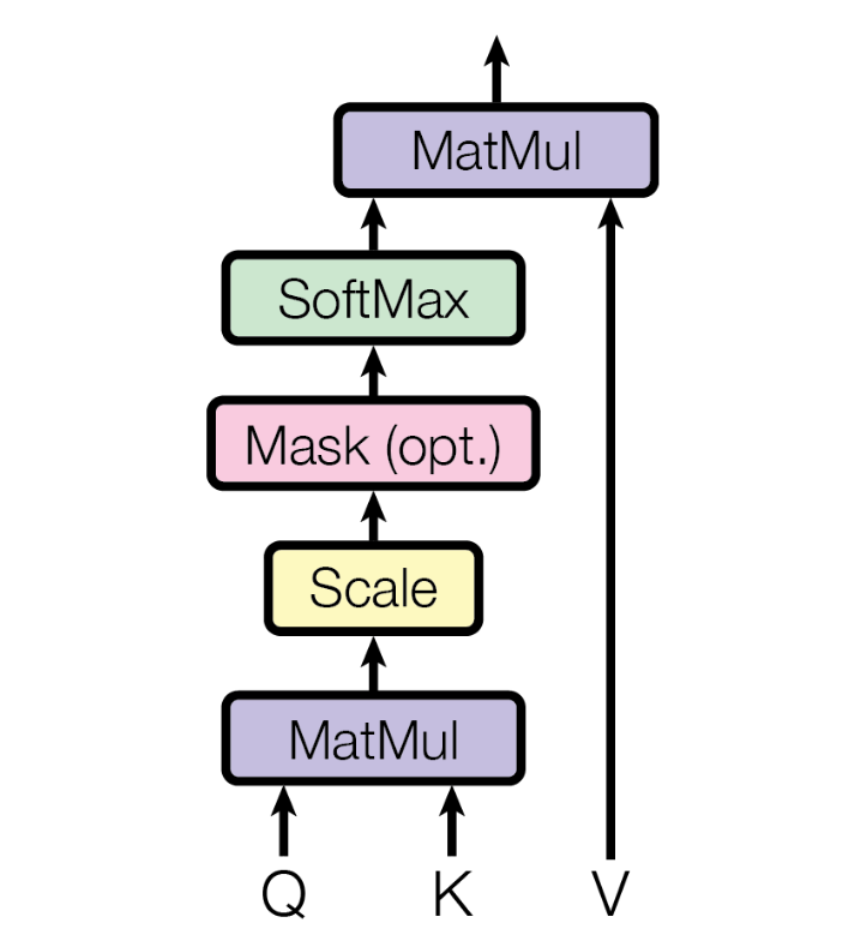
\includegraphics[width=.5\linewidth]{vaswani-attention}
                            \caption{\footnotesize Opmærksomhed [Vas+17]}
                    \end{figure}\noindent
                }
                \only<2->{
                    \begin{table}[H]
                    \begin{tabular}{c|c}
                        Entitet       & ID\\\hline
                        $\vdots$      & $\vdots$\\
                        New York City & \texttt 5\\
                        Christian 4.  & \texttt 6\\
                        $\vdots$      & $\vdots$
                    \end{tabular}
                    \caption{\footnotesize Entitets-ordforråd}
                    \end{table}
                }
            \end{overlayarea}
    \end{columns}
    \begin{example}
        \footnotesize
        \only<1>{
            \nw{Fredag}{1} \nw{rykkede}{2} Syd- og Sønderjyllands \nw{Politi}{3} ud til Sønderborg \nw{Lufthavn}{4}.
            \begin{tikzpicture}[overlay]
                \path[->,blue!60,thick](1) edge [out=-90, in=-90] (2);
                \path[->,blue,very thick](3) edge [out=-90, in=-90] (4);
            \end{tikzpicture}
        }
        \only<2>{
            \nw{Fredag}{1} \nw{rykkede}{2} \nw{Syd- og Sønderjyllands Politi}{3} ud til \nw{Sønderborg Lufthavn}{4}.
            \begin{tikzpicture}[overlay]
                \path[->,blue!60,thick](1) edge [out=-90, in=-90] (2);
                \path[->,red, very thick](3) edge [out=-90, in=-90] (4);
            \end{tikzpicture}
        }
    \end{example}
\end{frame}

\begin{frame}
    % 3
    \frametitle{En prætrænet, frit tilgængelig DaLUKE}
    \begin{columns}
        \column{0.33\textwidth}
        \begin{itemize}
            \item Trænet med ny softwarepakke
            \item Ingredienser
                \begin{itemize}
                    \item Dansk Wikipedia giver entiteter
                    \item Dansk BERT [Bot19] giver transformer
                    \item Gæt skjulte entiteter og ord $\times 150$ epoker
                \end{itemize}
        \end{itemize}

        \column{0.67\textwidth}
        \begin{figure}[H]
            \centering
            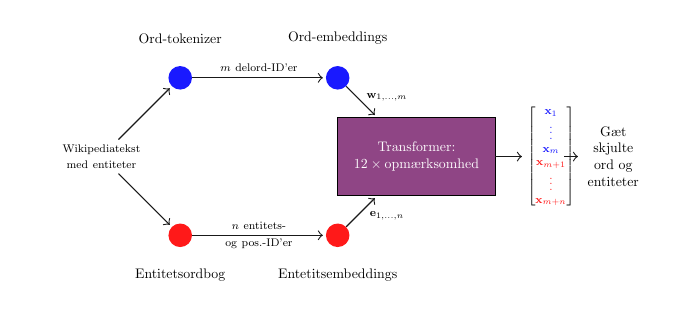
\begin{tikzpicture}[shorten >=1pt,->,draw=black!90, scale=0.5, every node/.style={scale=0.5}]
\tikzstyle{every pin edge}=[<-,shorten <=1pt]
\tikzstyle{path} = [ultra thick]
\tikzstyle{neuron}=[circle,fill=black!25,minimum size=17pt,inner sep=0pt]

\tikzstyle{shared neuron}=[neuron, fill=purple!90];
\tikzstyle{word neuron}=[neuron, fill=blue!90];
\tikzstyle{entity neuron}=[neuron, fill=red!90];

\tikzstyle{annot} = [text width=10em, text centered]

\node[annot] (I) at (-2, 0) {\footnotesize Wikipediatekst med entiteter};

\node[word neuron] (T-W) at (0, 2) {};
\node[entity neuron] (T-E) at (0, -2) {};
\node[annot, above of=T-W, node distance=1 cm] {Ord-tokenizer};
\node[annot, below of=T-E, node distance=1 cm] {Entitetsordbog};

\path (I) edge (T-W);
\path (I) edge (T-E);

\node[word neuron] (E-W) at (4, 2) {};
\node[entity neuron] (E-E) at (4, -2) {};
\node[annot, above of=E-W, node distance=1 cm] {Ord-embeddings};
\node[annot, below of=E-E, node distance=1 cm] {Entetitsembeddings};

\path (T-W) edge (E-W);
\path (T-E) edge (E-E);

\node[annot] at (2, 2.25) {\footnotesize $m$ delord-ID'er};
\node[annot, text width=5em] at (2, -2) {\footnotesize $n$ entitets- og pos.-ID'er};

\node[rectangle, draw = black,
    text = white,
    align=center,
    fill = Plum,
    minimum width = 4cm,
    minimum height = 2cm
    ] (T) at (6,0) {Transformer:\\\(12\times\text{opmærksomhed}\)};

\path (E-W) edge (T);
\path (E-E) edge (T);

\node[annot, text width=4em] at (5.25, 1.5) {\footnotesize $\mathbf w_{1, \ldots, m}$};
\node[annot, text width=4em] at (5.25, -1.5) {\footnotesize $\mathbf e_{1, \ldots, n}$};

\node[annot, text width=1em] at (9,0) {\footnotesize
    $\begin{bmatrix}
    \textcolor{blue!90}{\mathbf x_1}     \\
    \textcolor{blue!90}{\vdots}  \\
    \textcolor{blue!90}{\mathbf x_{m}}   \\
    \textcolor{red!90}{\mathbf x_{m+1}} \\
    \textcolor{red!90}{\vdots}  \\
    \textcolor{red!90}{\mathbf x_{m + n}}
    \end{bmatrix}
    $
};
\path (T) edge (8.75, 0);

\node[annot, text width=4em] (F) at (11, 0) {Gæt skjulte ord og entiteter};
\path (9.75, 0) edge (F);
\end{tikzpicture}

        \end{figure}\noindent
        \vspace{-1cm}
        \begin{example}
            \footnotesize
            \begin{overlayarea}{\textwidth}{1cm}
                \only<1>{
                Krøyer studerede på Kunstakademiet.
                }
                \only<2>{
                    $
                    \underbrace{\text{\textcolor{blue}{Krøyer}}}_{\mathclap{{\text{\textcolor{red}{P. S. Krøyer}}}}}
                    \ \text{\textcolor{blue}{studerede på}}
                    \ \underbrace{\text{\textcolor{blue}{Kunstakademiet}}}_{\mathclap{\text{\textcolor{red}{Det Kongelige Danske Kunstakademi}}}}
                    $.
                }
                \only<3>{
                    $
                    \underbrace{\text{\textcolor{blue}{Krøyer}}}_{\mathclap{{\text{\textcolor{red}{[MASK]}}}}}
                    \ \text{\textcolor{blue}{[MASK] på}}
                    \ \underbrace{\text{\textcolor{blue}{Kunstakademiet}}}_{\mathclap{\text{\textcolor{red}{Det Kongelige Danske Kunstakademi}}}}
                    $.
                }
            \end{overlayarea}
        \end{example}
    \end{columns}
\end{frame}

\section{Hvordan gik det?}
\begin{frame}
    \frametitle{Prætræningen}
    \begin{figure}[H]
        \centering
        \only<1>{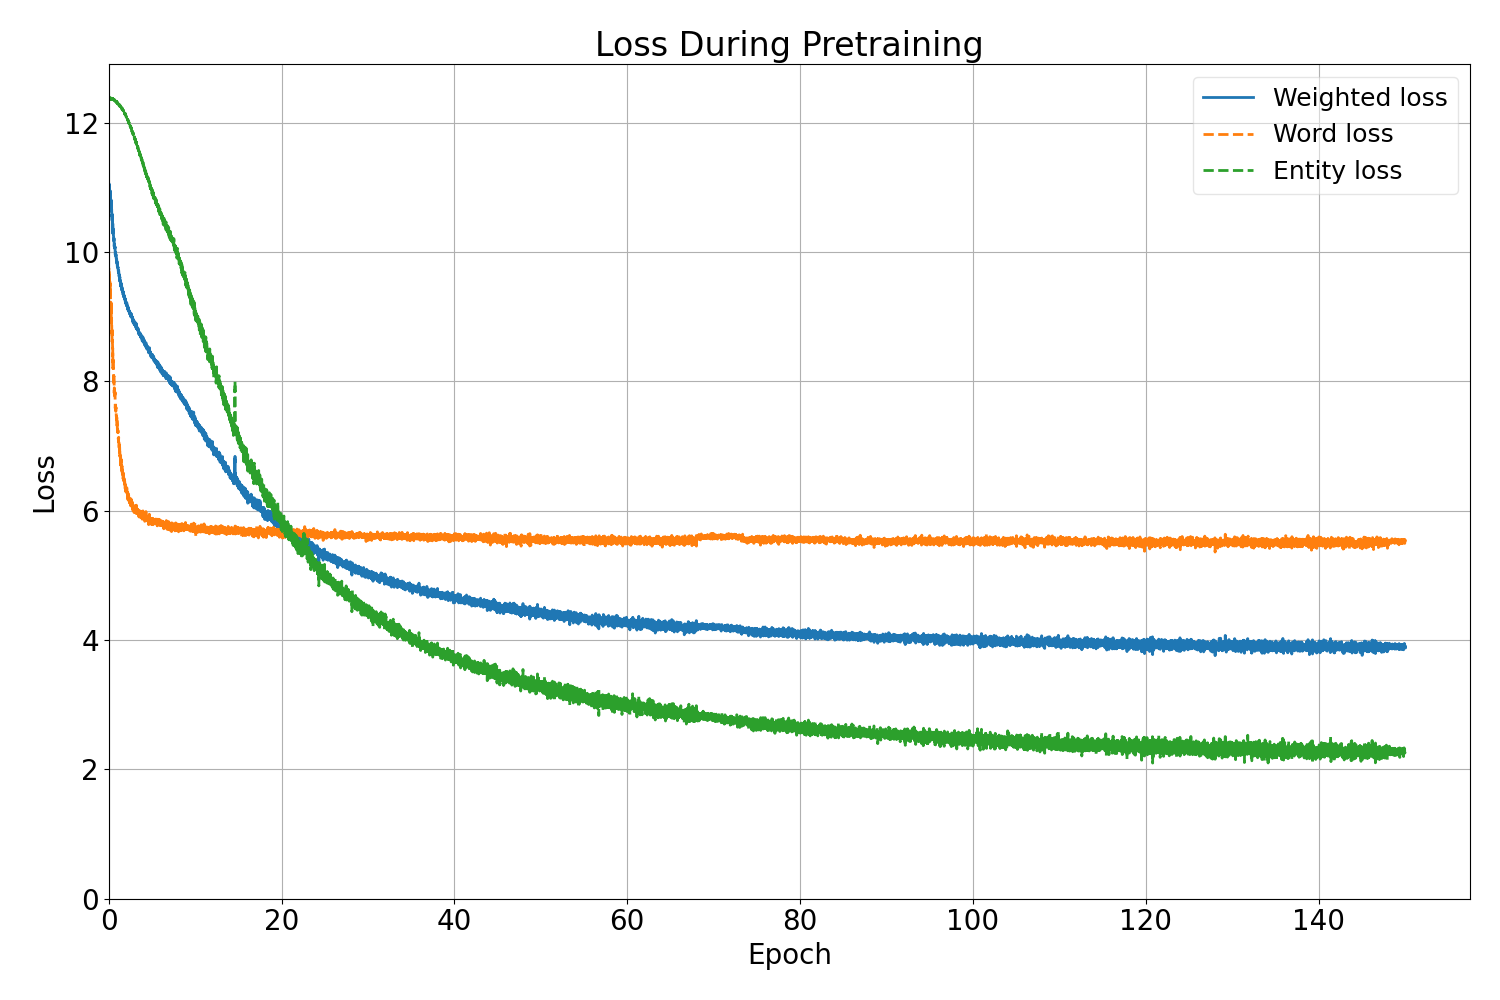
\includegraphics[width=.8\textwidth]{loss}}
        \only<2>{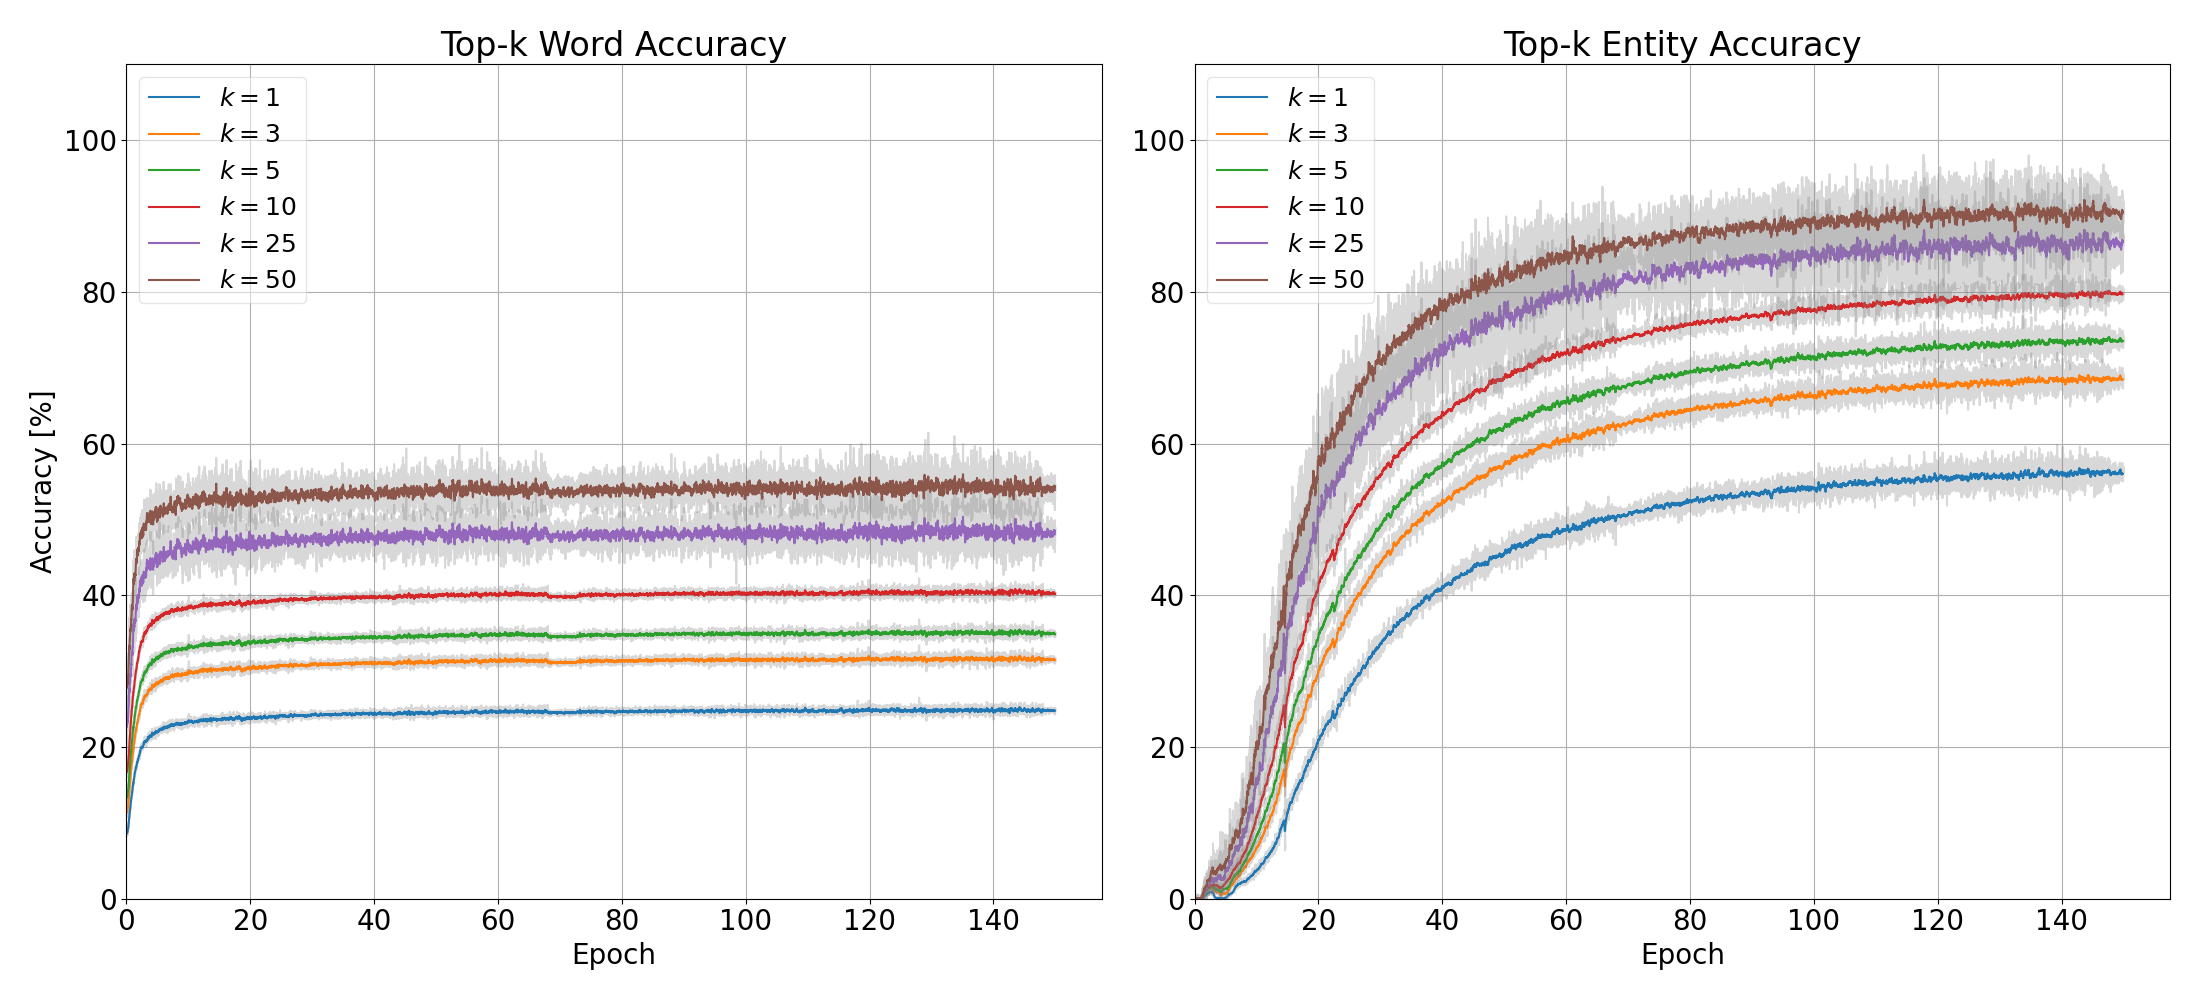
\includegraphics[width=\textwidth]{pretrain-acc}}
    \end{figure}\noindent
\end{frame}

\begin{frame}
    % 3
    \frametitle{NER på dansk}
    Primært datasæt: \emph{DaNE} med 5.512 annoterede sætninger, heraf $ \sim 10\pro $ til validering og $ \sim 10\pro $ til test
    \begin{columns}
        \column{0.45\textwidth}
        \begin{itemize}
            \item Fire kategorier: LOC, PER, ORG og MISC
            \item Optimerer hyperparametre på val. og giver den 15 epoker på træningssæt
            \item Model evalueres på valideringssæt efter hver epoke, og den bedste model gemmes
        \end{itemize}
        \column{0.55\textwidth}
        \begin{figure}[H]
            \centering
            \begin{overlayarea}{\textwidth}{4cm}
                \only<1>{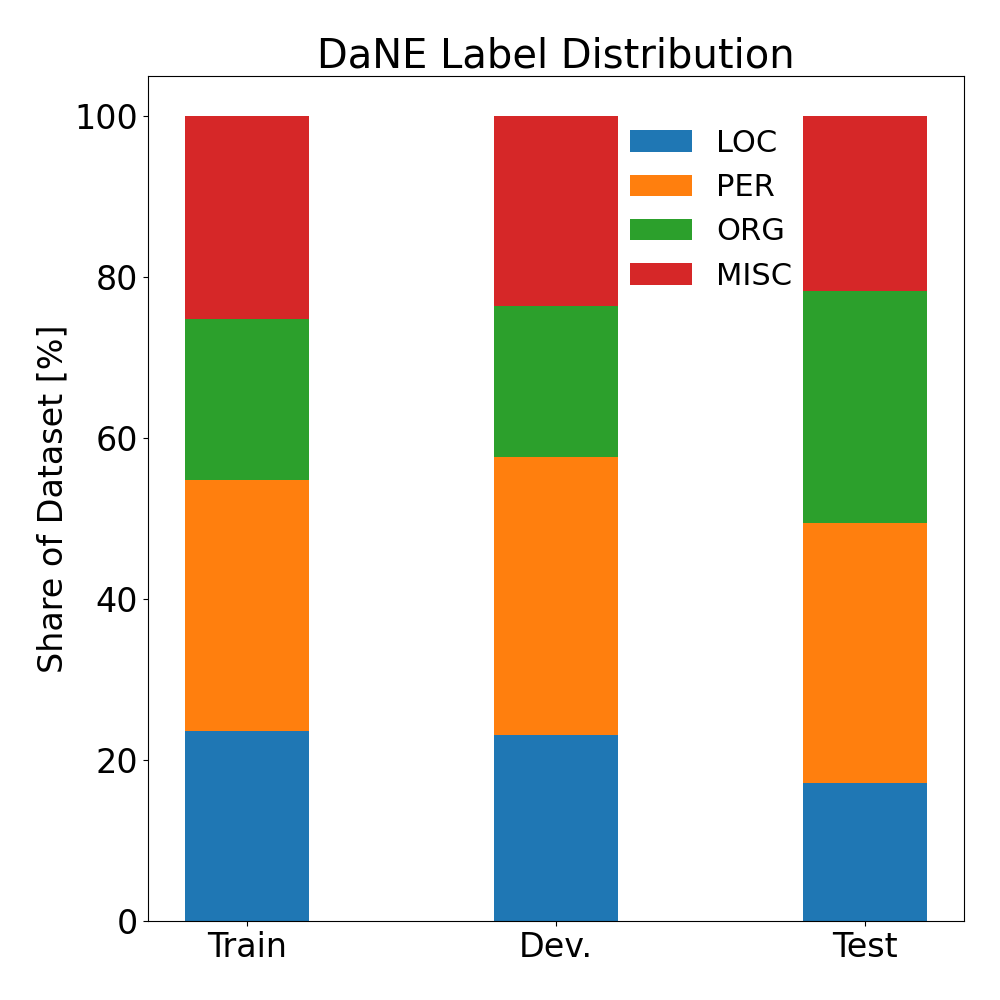
\includegraphics[width=0.8\textwidth]{datadist_dane}}
                \only<2>{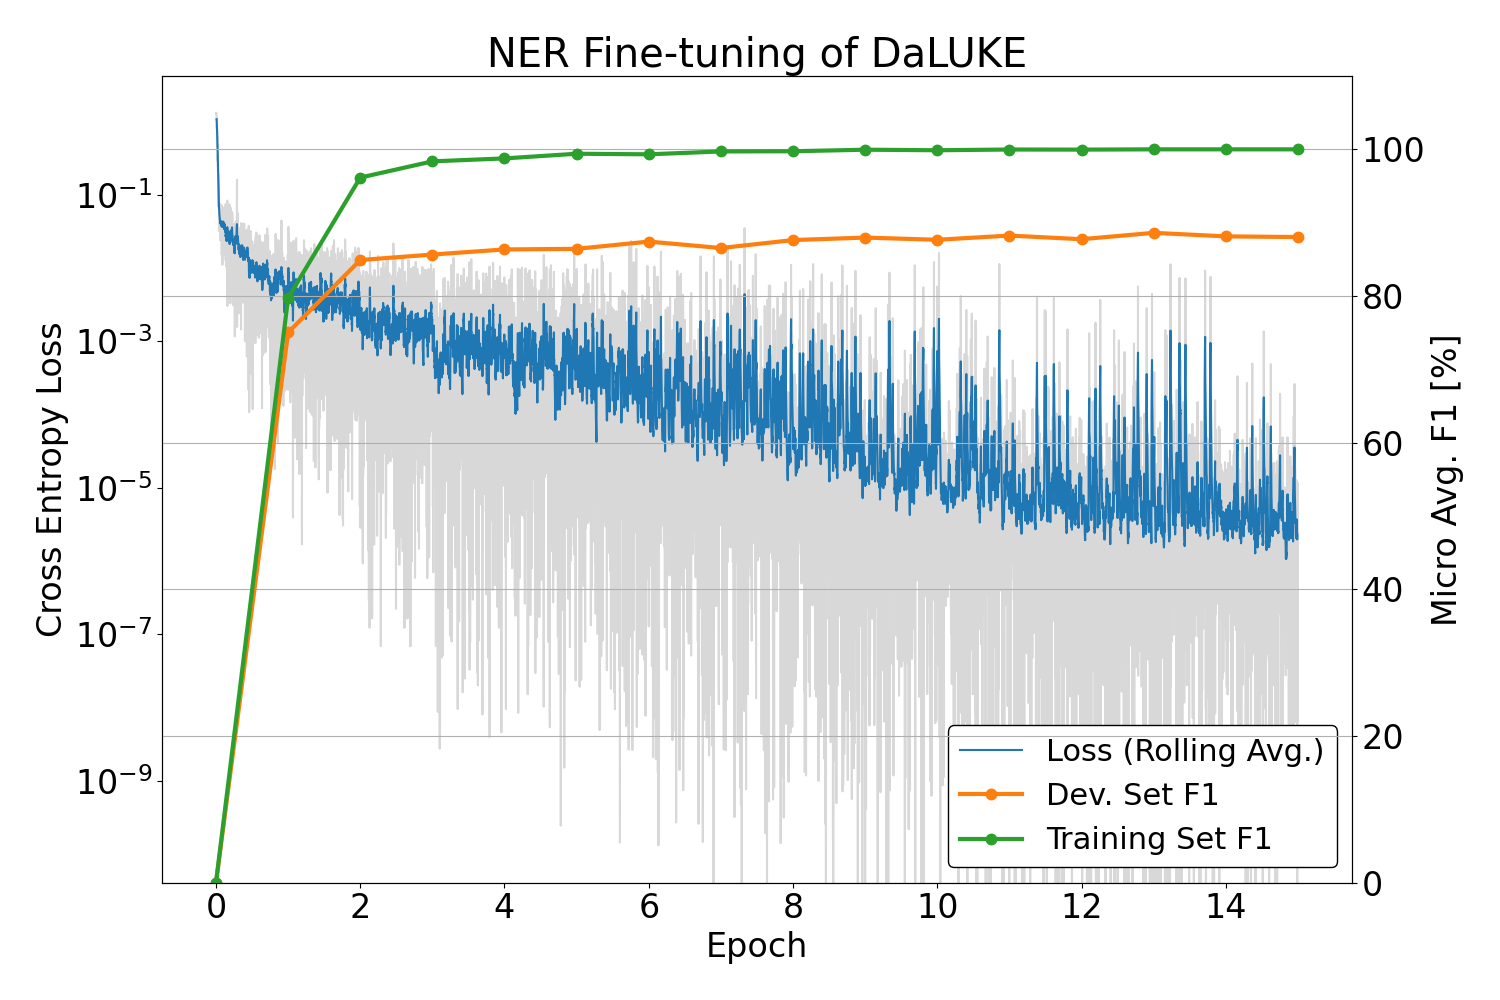
\includegraphics[width=\textwidth]{loss-fine}}
            \end{overlayarea}
        \end{figure}
    \end{columns}
\end{frame}

\begin{frame}
    \frametitle{NER på dansk}
    DaLUKE er den næstbedste danske NER-model på DaNE ved punktestimat
    \begin{table}[H]
        \fontsize{6pt}{8pt}\selectfont
            \begin{center}
                    \begin{tabular}{l l | c c c c | c c c c}
                        \multirow{2}{*}{Model} & \multirow{2}{*}{Trænet på} & \multicolumn{4}{c|}{Micro-middel [\pro]} & \multicolumn{4}{c}{Klasse-F1 [\pro]}\\
                        &         & F1                   & Prec.         & Rec.          & F1 {\tiny\textdiscount MISC} & LOC            & PER            & ORG            & MISC \\\hline
        DaLUKE        & DaNE      & 82.9 $\pm 3$         & 84.7          & 81.2          & 85.2         $\pm 3$         & \textbf{87.0} & \textbf{94.2} & 73.2          & 74.6 \\\hline
        DaNLP da-BERT & DaNE      & --                   & --            & --            & 84.0         $\pm 3$         & 83.9          & 92.8          & 73.0          & -- \\
        NERDA m-BERT  & DaNE      & 79.2 $\pm 3$         & 82.1          & 76.5          & 81.7         $\pm 4$         & 83.5          & 92.6          & 66.9          & 70.3 \\
        NERDA Ælæctra & DaNE      & 70.6 $\pm 4$         & 76.1          & 65.8          & 74.5         $\pm 4$         & 77.3          & 86.9          & 56.2          & 56.4 \\
        DaCy medium   & DaNE      & 78.3 $\pm 3$         & 78.3          & 78.3          & 80.5         $\pm 4$         & 84.0          & 90.4          & 66.2          & 70.1 \\
        DaCy large    & DaNE      & \textbf{84.9} $\pm 3$& \textbf{86.2} & \textbf{83.7} & \textbf{86.9} $\pm 3$         & 85.3          & \textbf{94.2} & \textbf{79.0} & \textbf{78.1} \\
        DaNLP spaCy   & DaNE      & 73.8 $\pm 4$         & 76.1          & 71.5          & 75.7         $\pm 4$         & 76.0          & 87.8          & 59.6          & 66.1 \\
        DaNLP Flair   & DaNE      & --                   & --            & --            & 81.8         $\pm 4$         & 84.8          & 93.2          & 63.0          & -- \\
        Polyglot      & Wikipedia & --                   & --            & --            & 64.2         $\pm 4$         & 65.0          & 78.7          & 39.3          & -- \\
        daner         & ITU DDT   & --                   & --            & --            & 56.5         $\pm 5$         & 59.4          & 70.4          & 28.3          & --
                    \end{tabular}
            \end{center}
    \end{table}
\end{frame}

\begin{frame}
    % 2
    \frametitle{NER-resultater er usikre}
    \begin{columns}
        \column{0.4\textwidth}
        \begin{itemize}
            \item 558 entiteter i testsæt $\Rightarrow \pm 3\pro$ på topresultater
            \item Udvælgelsesbias for parametriserede metoder
            \item<2-> Træningsprocessens indeterminisme giver også usikkerhed
            \item<3-> Datasættets fordeling ikke uden bias
        \end{itemize}
        \column{0.6\textwidth}
        \begin{figure}[H]
            \centering
            \begin{overlayarea}{\textwidth}{4cm}
                \only<2>{
                    \begin{table}[H]
                        \footnotesize
                        \centering
                        \begin{tabular}{l|ccc}
                            \multirow{2}{*}{Seed}  & \multicolumn{1}{c}{F1 [\pro]} & Præcision [\pro]               & Recall [\pro]               \\
                                               & Avg.  & Avg.                          & Avg.                        \\ \hline
                        1                      & 83.7  & 88.7                          & 79.2                        \\
                        2                      & 81.5  & 83.9                          & 79.3                       \\
                        3                      & 84.5  & 86.9                          & 82.2                       \\
                        4                      & 81.3  & 83.8                          & 79.0                       \\
                        5                      & 82.4  & 84.9                          & 80.1                       \\\hline
                        Middel                 & 82.7  & 85.6& 80.0\\
                        Std.                   & 1.4   & 2.1& 1.3
                        \end{tabular}
                        \caption{RNG-tilfældighed}
                    \end{table}\noindent
                }
                \only<3>{
                    \begin{table}[H]
                        \footnotesize
                        \centering
                        \begin{tabular}{l|ccc}
                            \multirow{2}{*}{Del}  & \multicolumn{1}{c}{F1 [\pro]} & Præcision [\pro]               & Recall [\pro]               \\
                                                & Avg. & Avg.                           & Avg.                        \\ \hline
                                        1     &  89.1 & 89.8 & 88.5\\
                                        2     &  86.1 & 88.2 & 88.1\\
                                        3     &  86.9 & 88.3 & 85.5\\
                                        4     &  87.4 & 87.8 & 87.1\\
                                        5     &  87.6 & 88.1 & 87.1\\\hline
                                        Middel&  87.4 & 88.4 & 87.3\\
                                        Std.  &  1.1  & 0.8  & 1.7
                        \end{tabular}
                        \caption{
                            Tilfældighed i datasæt-opdeling
                        }
                    \end{table}\noindent
                }
                \only<4>{
                    \begin{figure}[H]
                    \centering
                    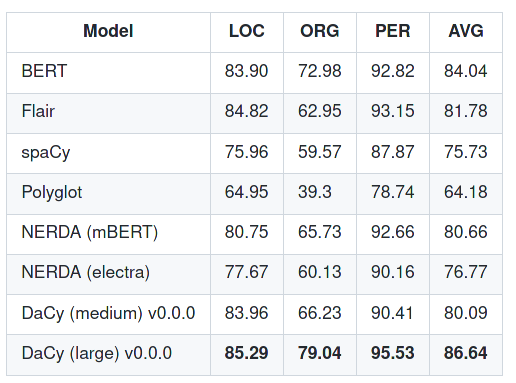
\includegraphics[width=.6\textwidth]{danlp-tab}
                        \caption{Resultater fra DaNLP [Bro+21]. Er lignende for DaNE [Hvi+20]}
                    \end{figure}\noindent
                }
            \end{overlayarea}
        \end{figure}
    \end{columns}
\end{frame}
\begin{frame}
    % 3
    \frametitle{Entitetsbevidst selvopmærksomhed}
    \tikzstyle{every picture}+=[remember picture]
    \tikzstyle{every path}=[<-,shorten <=1pt]
    \begin{itemize}
        \item Transformerudvidelse, der modellerer entitets-entitets- og ord-entitets-forhold direkte
        \item{} [Yam+20] viser bedre resultater i fine-tuningsopgaver
        \item Uden brug i prætræning falder fine-tuningsresultater med 2,8 procentpoint
    \end{itemize}
    \begin{example}
        \footnotesize
        \nw{Fredag}{1} \nw{rykkede}{2} \nw{Syd- og Sønderjyllands Politi}{3} ud til \nw{Sønderborg Lufthavn}{4}.
        \begin{tikzpicture}[overlay]
            \path[->,blue!60,thick](1) edge [out=-90, in=-90] (2);
            \path[->,red, very thick](3) edge [out=-90, in=-90] (4);
            \path[->,purple!80, very thick](2) edge [out=-90, in=-90] (3);
            \path[->,purple!80, very thick](3) edge [out=-90, in=-90] (1);
        \end{tikzpicture}
    \end{example}
\end{frame}

\begin{frame}
    % 2
    \frametitle{Transferlæring}
    \begin{columns}
        \column{0.4\textwidth}
        \begin{itemize}
            \item Hvad hvis man ikke initialiserede fra den danske BERT?
            \item Langt bedre præcision i prætræning - tyder på overfitting
            \item Fine-tuning ligger 11,4 procentpoint under baseline
            \item Transferlæring virker stabiliserende og regulariserende
        \end{itemize}
        \column{0.6\textwidth}
        \begin{figure}[H]
            \centering
            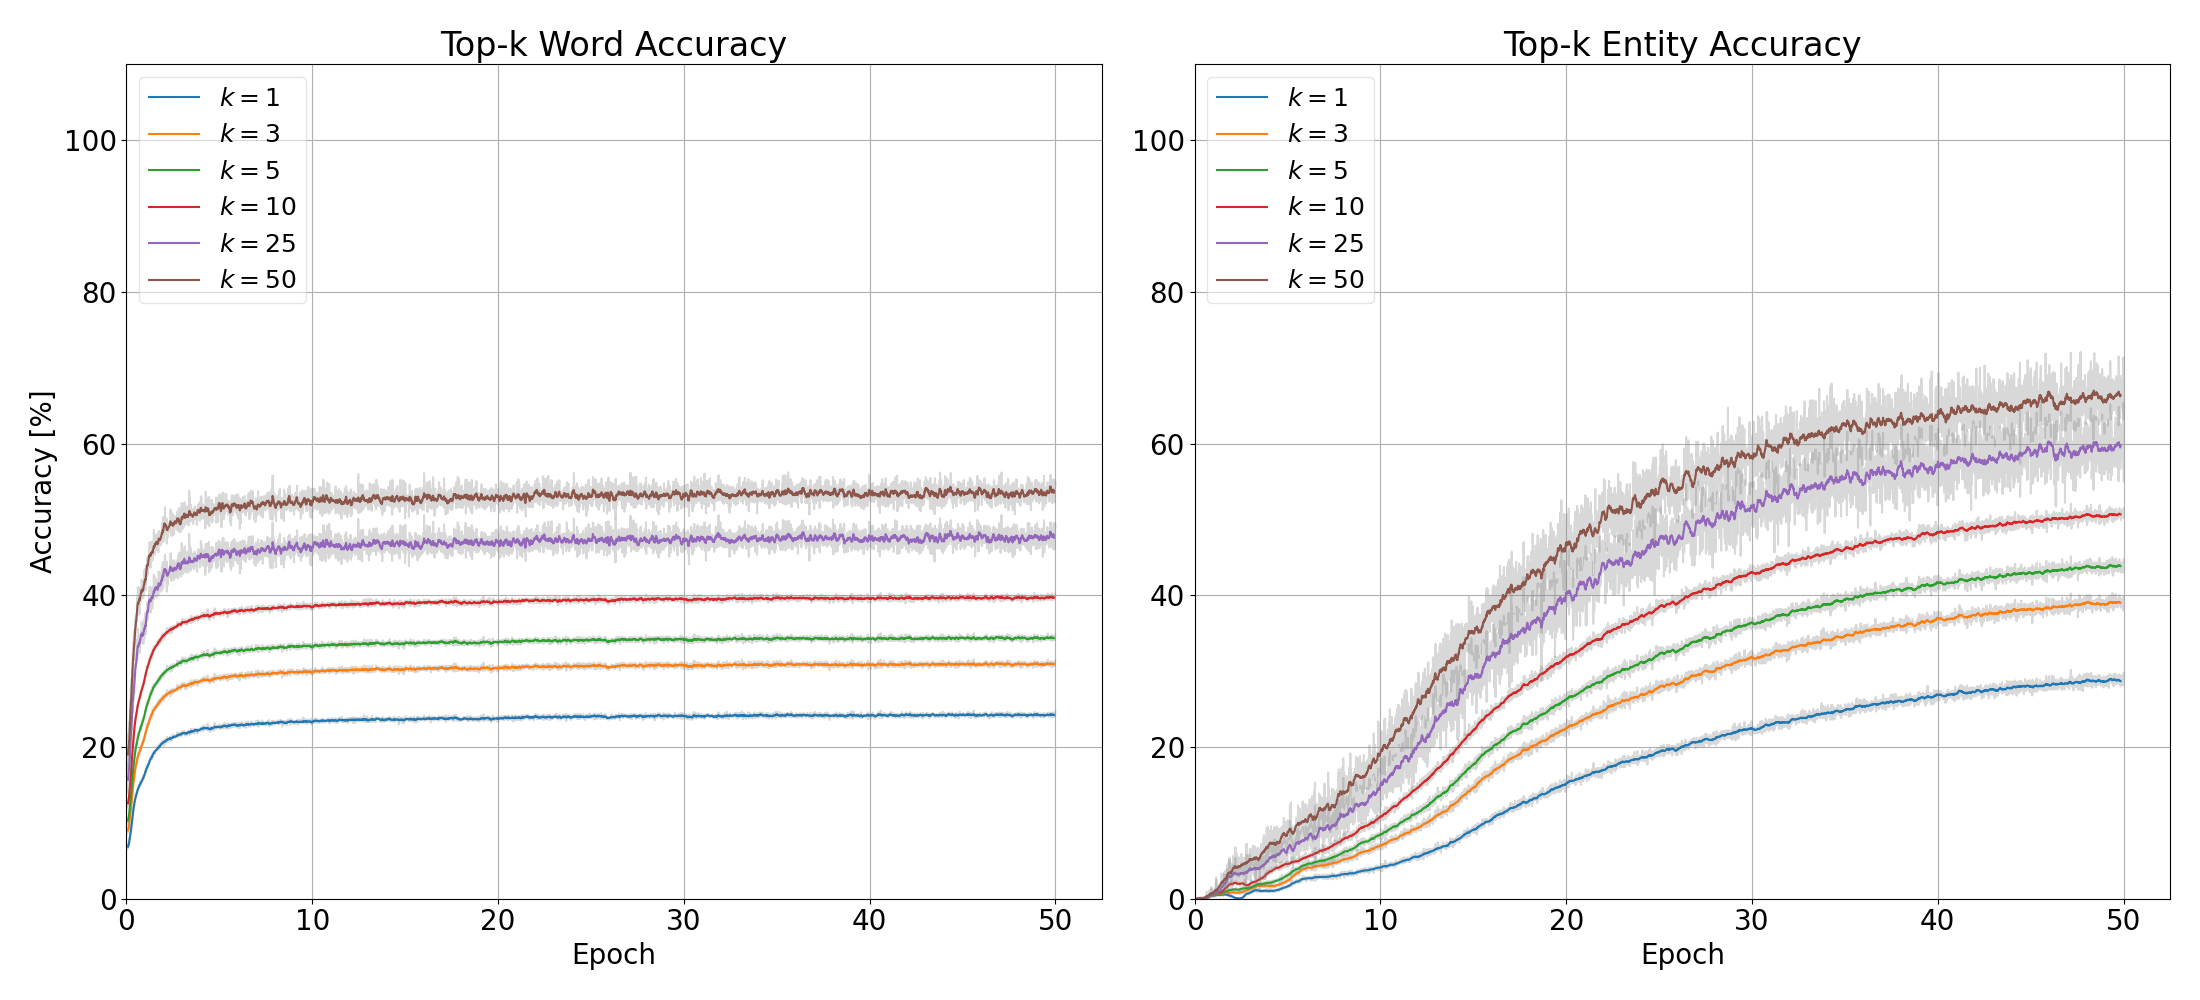
\includegraphics[width=.85\textwidth]{baseline-acc}
            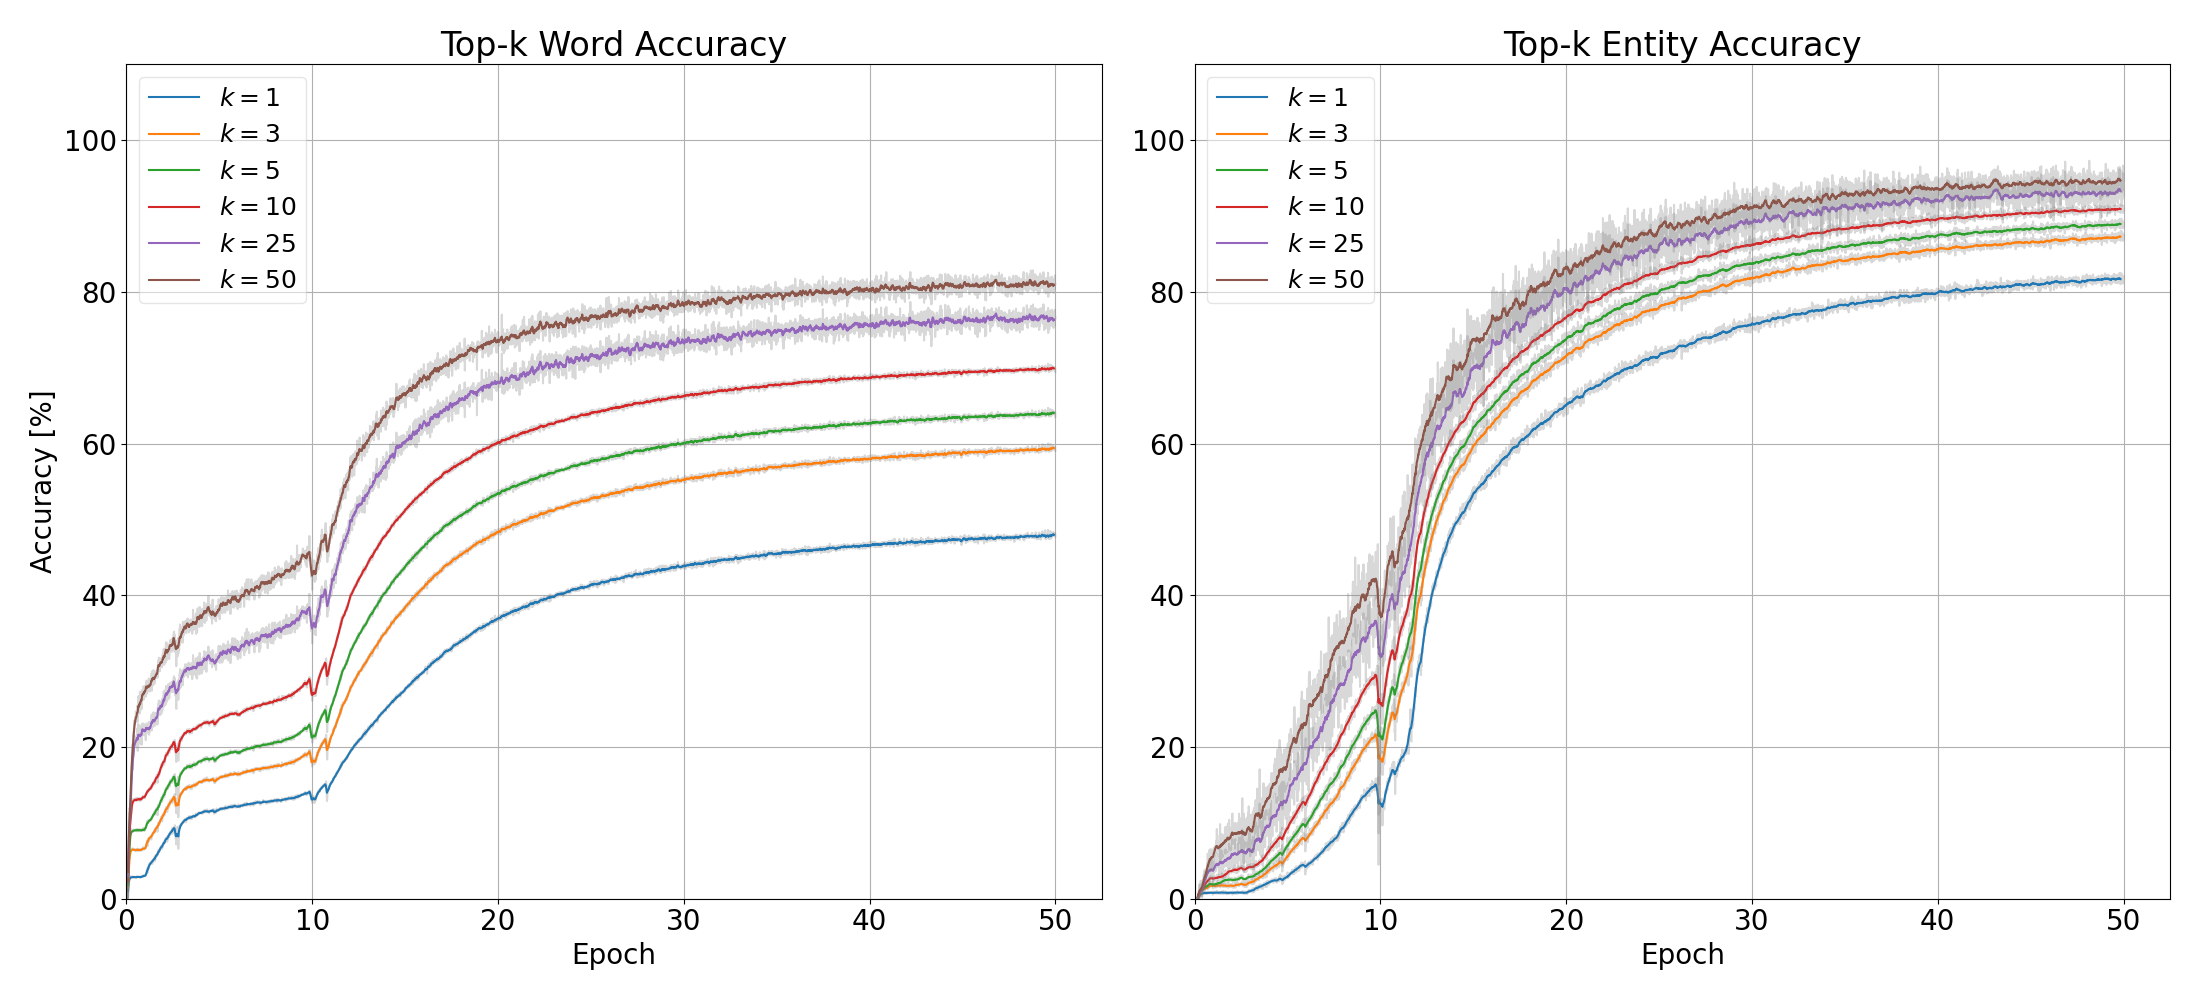
\includegraphics[width=.85\textwidth]{nobert-acc}
            \caption{Øverst: Baseline. Nederst: Ingen transferlæring}
        \end{figure}\noindent
    \end{columns}
\end{frame}

\begin{frame}
    % 2
    \frametitle{Datasætmodifikationer}
    \begin{itemize}
        \item Datasæt udvides med ekstra entiteter automatisk: $ 47\pro $ flere
        \item Uden dem fås 0,6 procentpoint højere
        \item I LUKE beskæres entitetsordforrådet til de mest brugte. Hvilken effekt har det i DaLUKE?
        \item 0,2 procentpoint lavere med færre entiteter
    \end{itemize}
    \begin{example}
        "Arkæologi er studiet af tidligere tiders {\color{red}menneske}lige {\color{red}aktivitet}, primært gennem studiet af {\color<2>{blue}menneske}ts materielle levn. Langt det meste af al {\color<2>{blue}menneske}lig {\color<2>{blue}aktivitet} foregik, før vi lærte at skrive, så {\color<2>{blue}arkæologi} er den vigtigste metode til at studere ældre {\color<2>{blue}menneske}skabte samfund."
    \end{example}
\end{frame}

\section{Hvad har vi lært?}
\begin{frame}
    \frametitle{Modellens sandsynligheder}
    \begin{figure}[H]
        \centering
            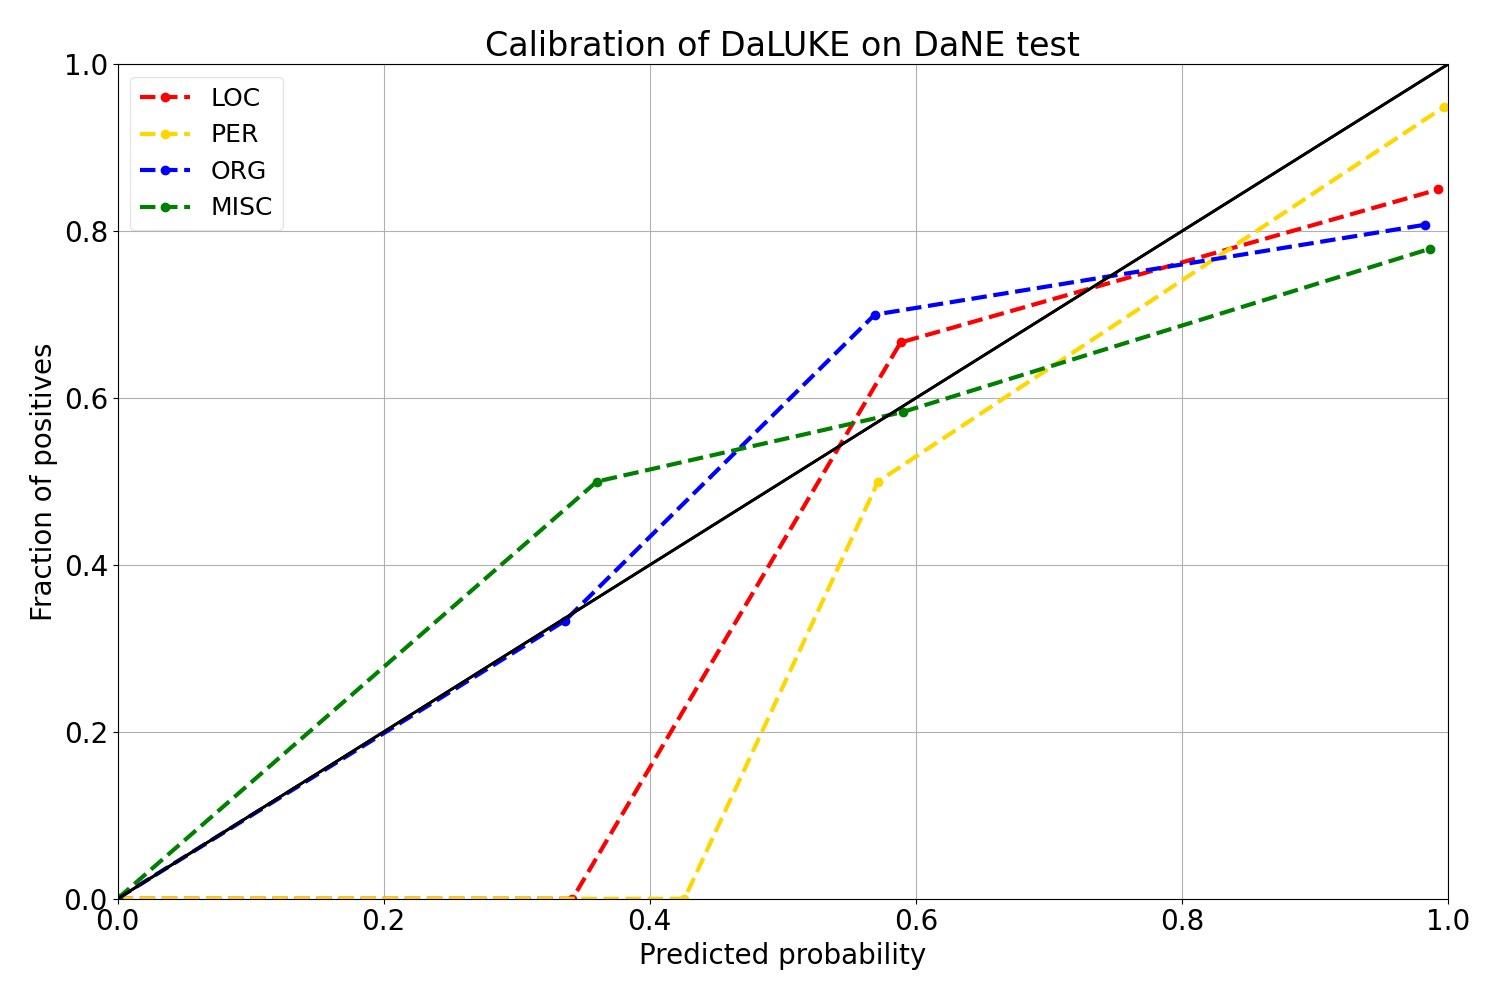
\includegraphics[width=.8\linewidth]{calibration}
    \end{figure}\noindent
\end{frame}

\begin{frame}
    % 3
    \frametitle{Vektorer fanger sprogforståelse}
    \begin{itemize}
        \only<1-7>{\item Prætrænet model indeholder sproglig struktur}
        \only<8->{\item Fine-tuning tilpasser vektorer til opgaven \only<9>{-- også på test.}}
    \end{itemize}
    \begin{figure}[H]
        \centering
        \only<1>{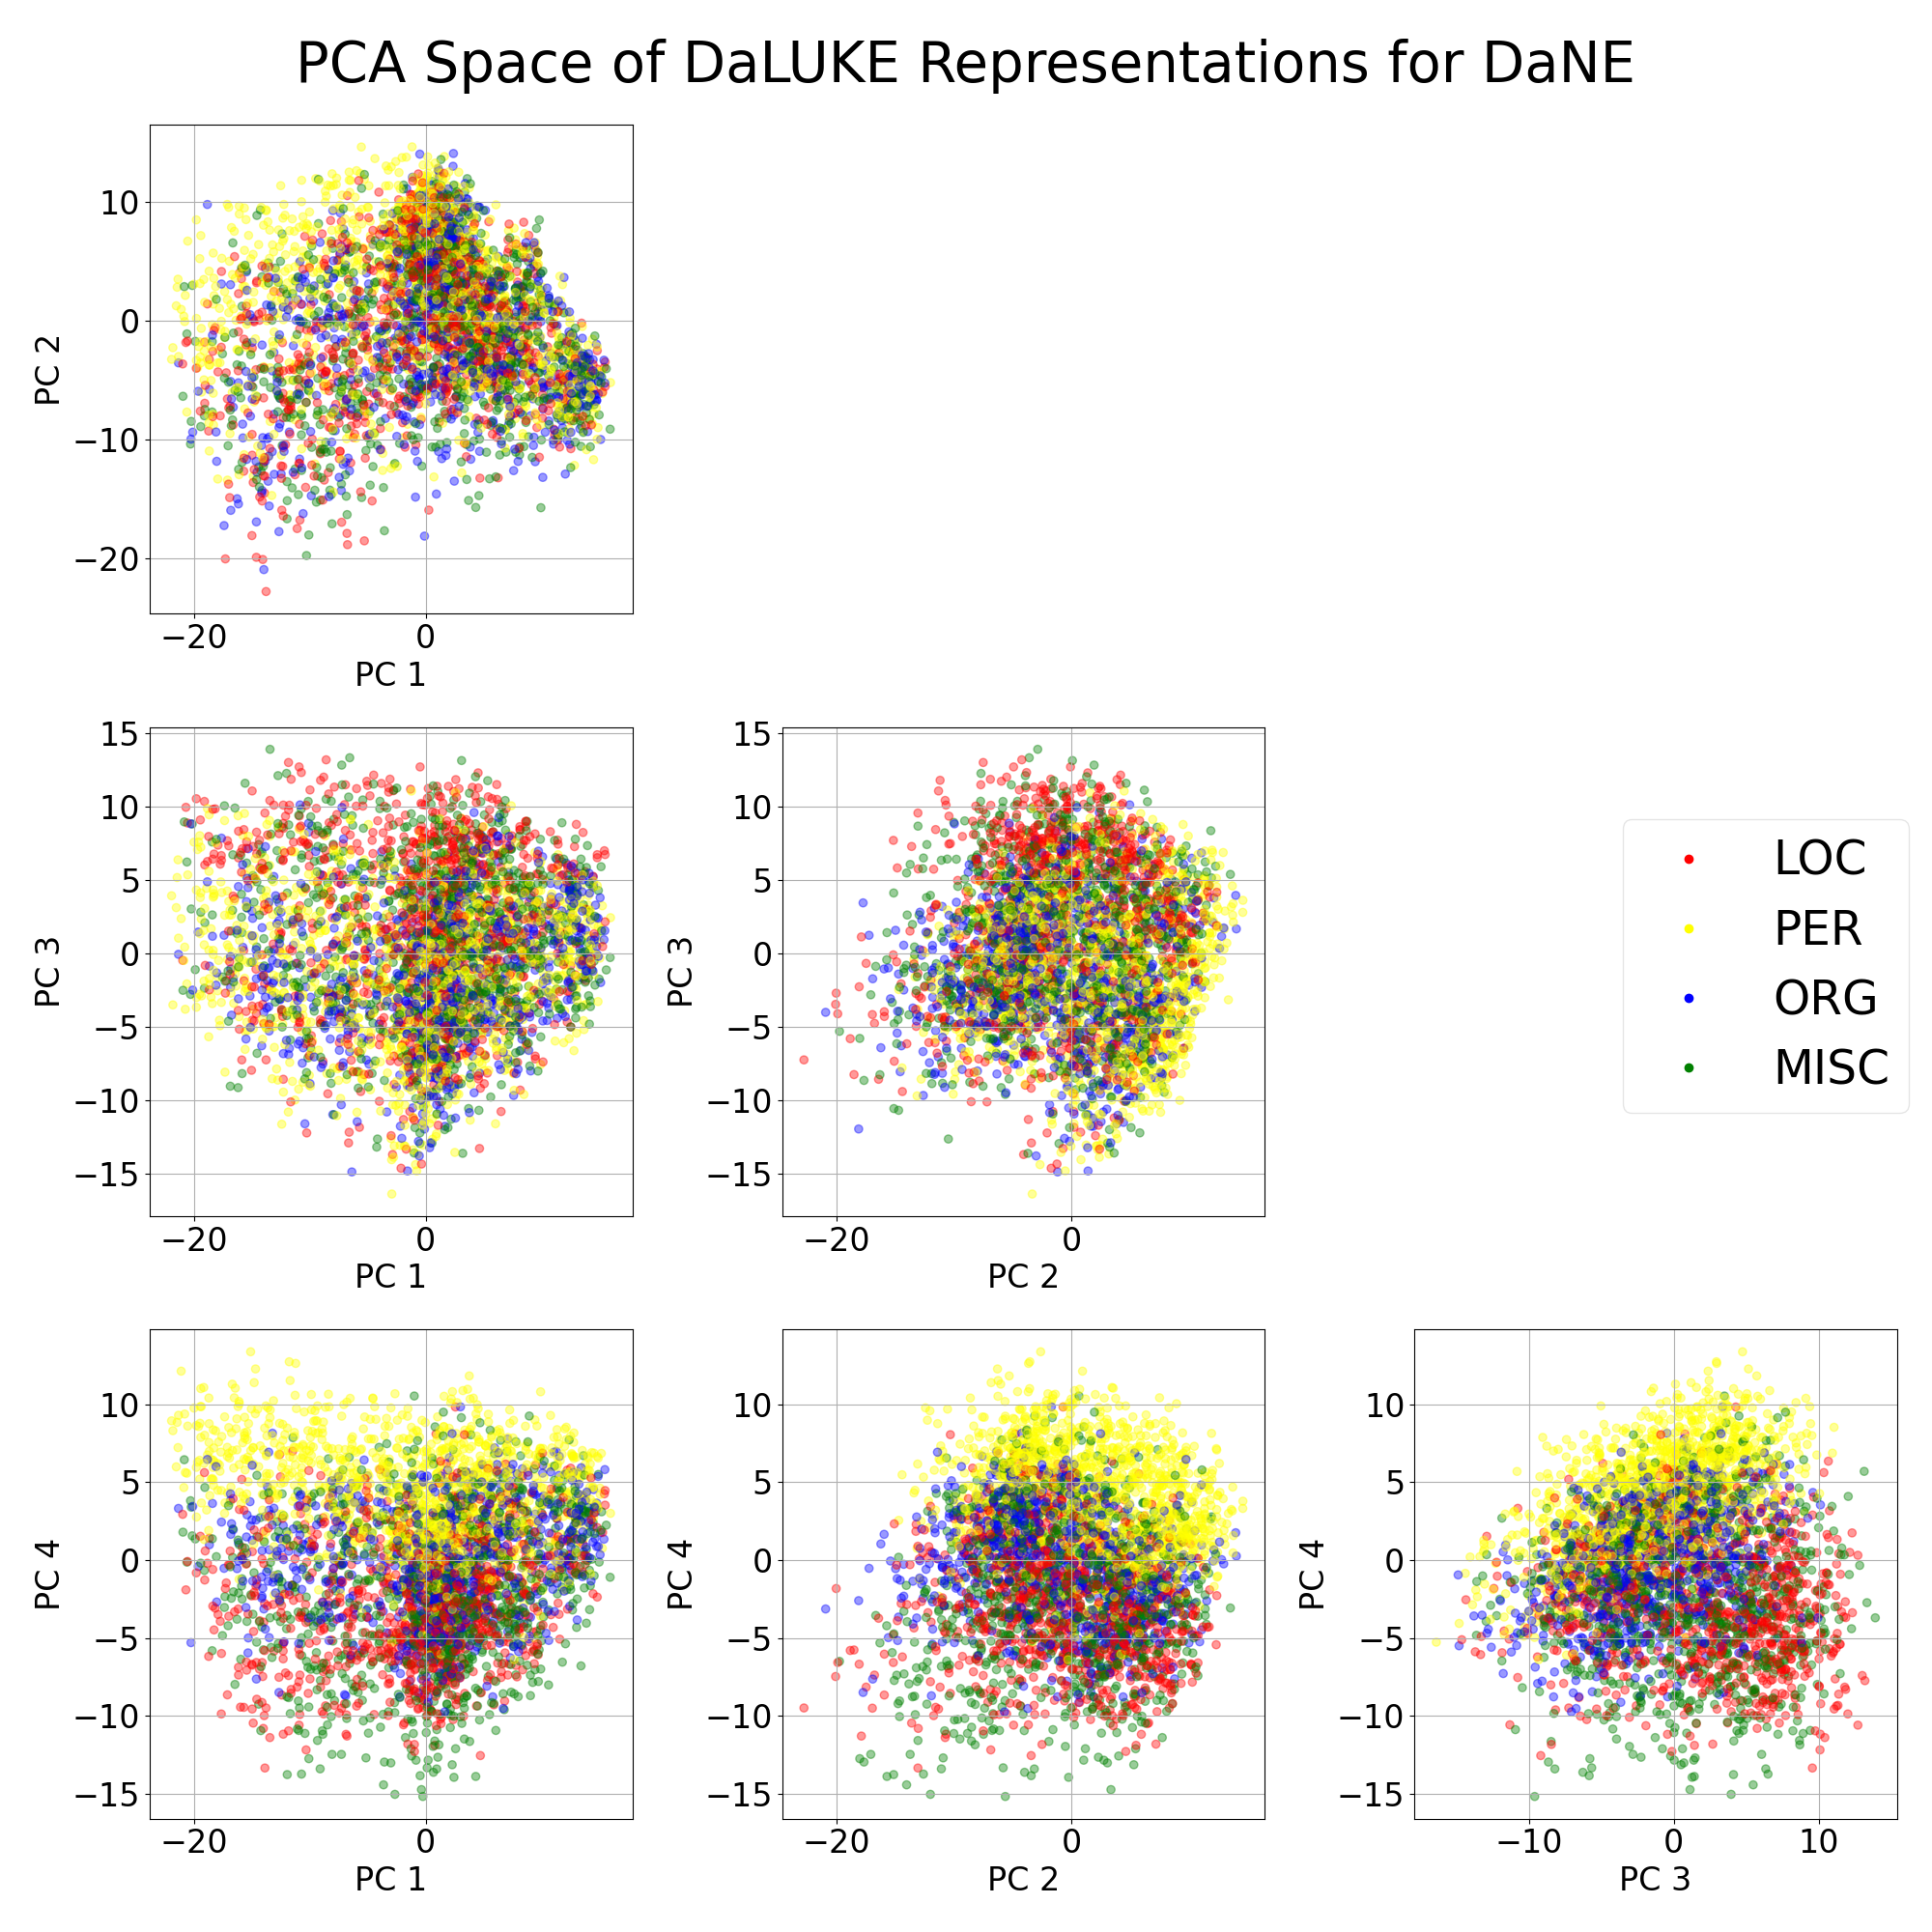
\includegraphics[width=.5\linewidth]{pos-geo/pca_matrix}}
        \only<2->{
            \begin{tikzpicture}
                \node[above right, inner sep=0] (image) at (0,0) {
                    \includegraphics<2-7>[width=.8\linewidth]{pos-geo/umap}
                    \includegraphics<8>[width=.8\linewidth]{umap-finetuned}
                    \includegraphics<9>[width=.8\linewidth]{umap-finetuned-test}
                };
            % Create scope with normalized axes
                \begin{scope}[
                    x={($0.1*(image.south east)$)},
                    y={($0.1*(image.north west)$)}]

                    % % Grid
                    % \draw[lightgray,step=1] (image.south west) grid (image.north east);

                    % % Axes' labels
                    % \foreach \x in {0,1,...,10} { \node [below] at (\x,0) {\x}; }
                    % \foreach \y in {0,1,...,10} { \node [left] at (0,\y) {\y};}

                \draw<3-7>[stealth-, thick, black] (2.5,8.5) -- ++(0.5,0.25)
                    node[right,black,fill=white]{\small Danmark};
                \draw<4-7>[stealth-, thick, black] (4.7, 8.2) -- ++(0.5,0)
                    node[right,black,fill=white]{\small København};
                \draw<5-7>[stealth-, thick, black] (6.3, 7) -- ++(0.5,0)
                    node[right,black,fill=white]{\small EF};
                \draw<6-7>[stealth-, thick, black] (6.8, 3) -- ++(0.5,0)
                    node[right,black,fill=white]{\small Hafnia};
                \draw<7-7>[stealth-, thick, black] (5.8, 1.8) -- ++(0.5,0)
                    node[right,black,fill=white]{\small Balkan};
                \end{scope}
            \end{tikzpicture}
        }
    \end{figure}\noindent
\end{frame}

\begin{frame}
    % 3
    \frametitle{Kontekst og viden i modellen}
    \begin{columns}
        \column{0.5\textwidth}
    \begin{itemize}
        \uncover<1->{\item Modellen bruger fakta fra hele sætningen til forudsigelse}
        % \uncover<4->{\item Entitetsannoteringer gør det lettere at gætte skjulte ord}
        \uncover<4->{\item Entitetstype afhænger af kontekst}
    \end{itemize}
        \column{0.5\textwidth}
    \begin{example}
        \footnotesize
        \only<1-3>{
        ''
        Professor i astrofysik, \emph{[MASK] [MASK]}, udtaler til avisen, at den nye måling sandsynligvis ikke er en fejl. Observationen af dobbeltstjerne-systemet var usædvanlig klar og foregik over længere tid.
        \temporal<2>{Han}{\textbf{Hun}}{\textbf{Han}}
        har i sine 30 år på
        \alt<3>{\textbf{Harvard University}}{Københavns Universitet}
        ikke set noget lignende.
        ''
        \begin{itemize}
            \only<1>{\item Bo Møller, Peter Møller, Jakobsen}
            \only<2>{\item Bente Møller, Katrine Møller, Mette Holm}
            \only<3>{\item Peteran, Michael Brown, John Brown}
        \end{itemize}
        }
        \only<4>{
            ''\textbf{Det Kgl. Bibliotek} forvalter Danmarks største tekstsamling, der strækker sig fra middelalderen til det nyeste litteratur.''
        \begin{itemize}
            \item ORG
        \end{itemize}
            ''Du kan tage havnebussen til \textbf{Det Kgl. Bibliotek} og så tage videre med bussen.''
         \begin{itemize}
             \item LOC
         \end{itemize}
        }
    \end{example}
    \end{columns}
\end{frame}

\begin{frame}
    % 1
    \frametitle{Vejen til AI, der forstår dansk}
    \begin{columns}
        \column{0.5\textwidth}
        \begin{itemize}
            \item Viden som løsning på dataknaphed?
            \item Brugbar og god til NER
            \item Forbedringspotentiale
        \begin{figure}[H]
            \centering
                \href{https://github.com/peleiden/daLUKE}{
                    
\includegraphics[width=.7\linewidth]{daluke-mascot}
                }
        \end{figure}\noindent
        \end{itemize}
        \column{0.5\textwidth}
        \begin{figure}[H]
            \centering
                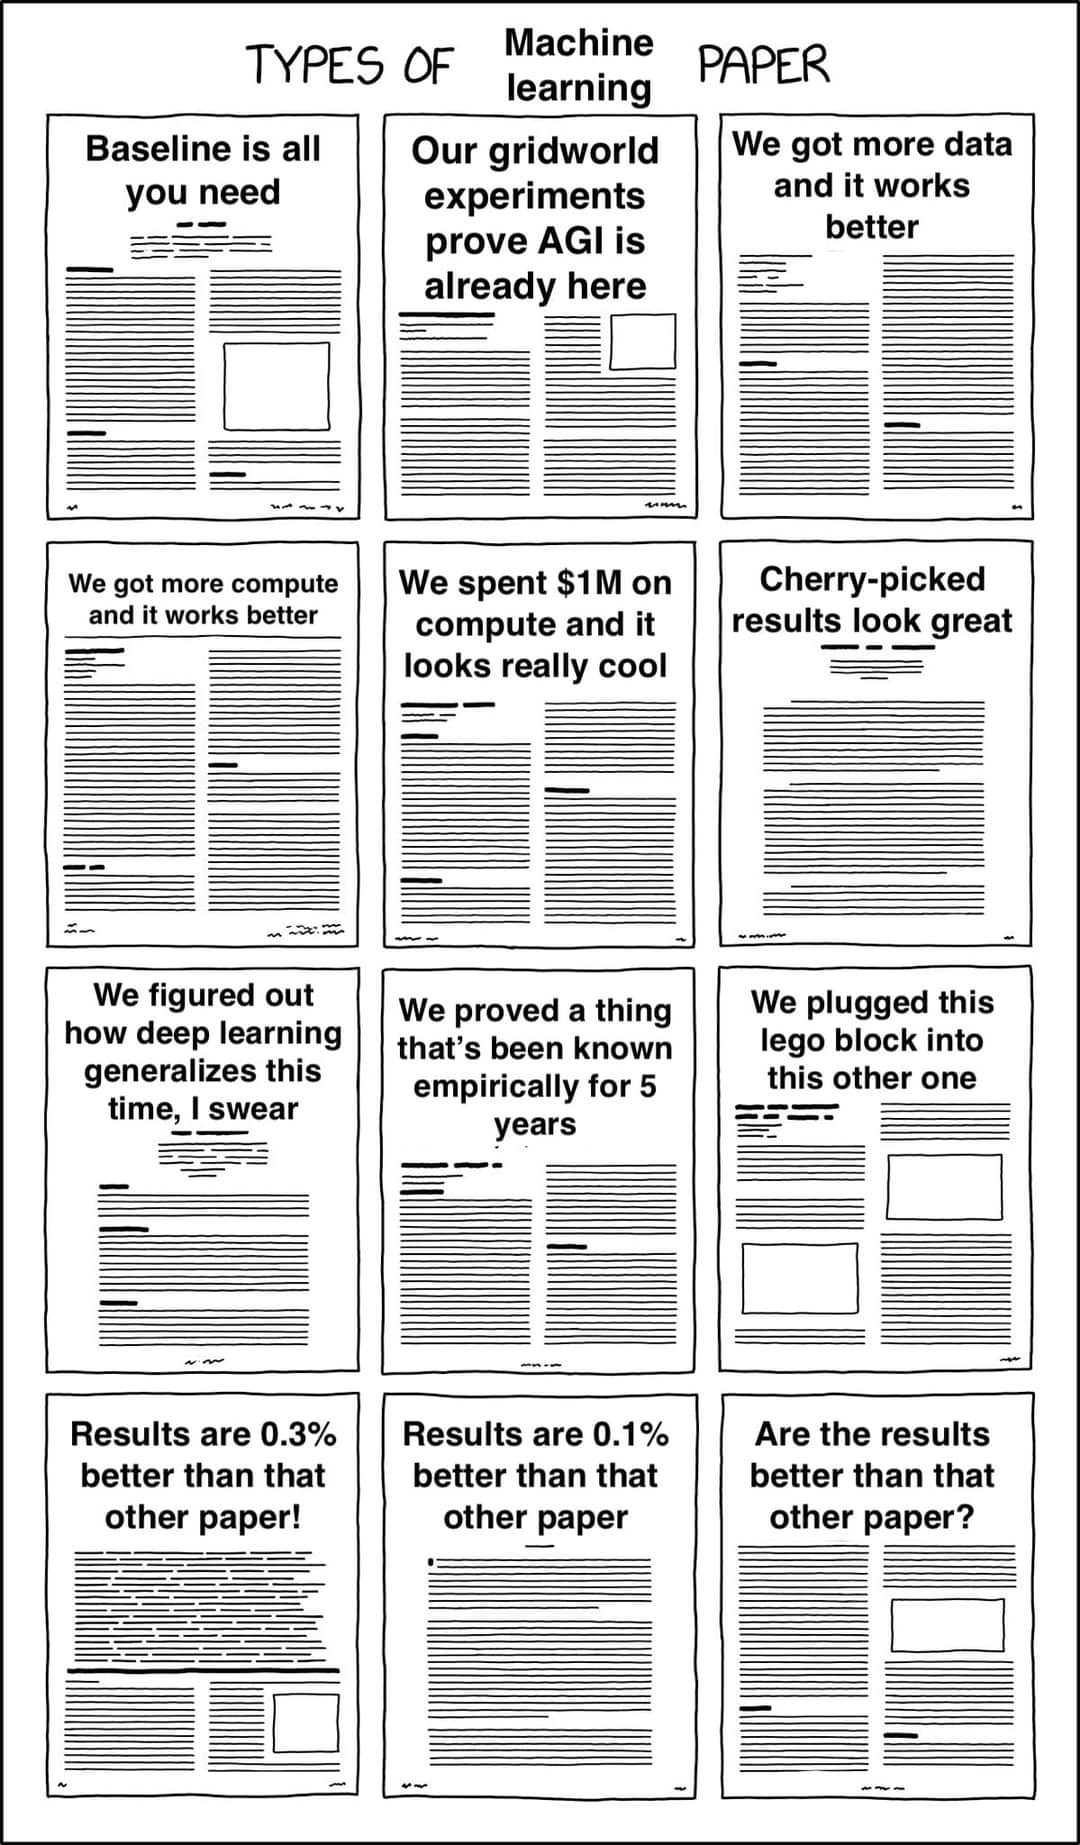
\includegraphics[width=.7\linewidth]{types-of-m}
        \end{figure}\noindent
    \end{columns}
\end{frame}

\end{document}
